\documentclass[10pt,twocolumn]{article}

% use the oxycomps style file
\usepackage{oxycomps}
\usepackage{dsfont}

%Some Greek letters

\def\a{\alpha}
\def\b{\beta}
\def\g{\gamma}
\def\G{\Gamma}
\def\d{\delta}
\def\D{\Delta}
\def\e{\epsilon}
\def\h{\theta}
\def\k{\kappa}
\def\l{\lambda}
\def\L{\Lambda}
\def\s{\sigma}
%\def\S{\Sigma}
\def\o{\omega}
\def\O{\Omega}

%Blackboard Bold

\newcommand{\bbC}{\mathds{C}}
\newcommand{\bbF}{\mathds{F}}
\newcommand{\bbN}{\mathds{N}}
\newcommand{\bbO}{\mathds{O}}
\newcommand{\bbQ}{\mathds{Q}}
\newcommand{\bbR}{\mathds{R}}
\newcommand{\bbZ}{\mathds{Z}}

%Mathcal

\newcommand{\mA}{\mathcal{A}}
\newcommand{\mB}{\mathcal{B}}
\newcommand{\mC}{\mathcal{C}}
\newcommand{\mD}{\mathcal{D}}
\newcommand{\mE}{\mathcal{E}}
\newcommand{\mF}{\mathcal{F}}
\newcommand{\mG}{\mathcal{G}}
\newcommand{\mH}{\mathcal{H}}
\newcommand{\mI}{\mathcal{I}}
\newcommand{\mJ}{\mathcal{J}}
\newcommand{\mK}{\mathcal{K}}
\newcommand{\mL}{\mathcal{L}}
\newcommand{\mM}{\mathcal{M}}
\newcommand{\mN}{\mathcal{N}}
\newcommand{\mO}{\mathcal{O}}
\newcommand{\mP}{\mathcal{P}}
\newcommand{\mQ}{\mathcal{Q}}
\newcommand{\mR}{\mathcal{R}}
\newcommand{\mS}{\mathcal{S}}
\newcommand{\mT}{\mathcal{T}}
\newcommand{\mU}{\mathcal{U}}
\newcommand{\mV}{\mathcal{V}}
\newcommand{\mW}{\mathcal{W}}
\newcommand{\mX}{\mathcal{X}}
\newcommand{\mY}{\mathcal{Y}}
\newcommand{\mZ}{\mathcal{Z}}


%mathfrak (missing \fi)

\newcommand{\fa}{\mathfrak{a}}
\newcommand{\fA}{\mathfrak{A}}
\newcommand{\fb}{\mathfrak{b}}
\newcommand{\fB}{\mathfrak{B}}
\newcommand{\fc}{\mathfrak{c}}
\newcommand{\fC}{\mathfrak{C}}
\newcommand{\fd}{\mathfrak{d}}
\newcommand{\fD}{\mathfrak{D}}
\newcommand{\fe}{\mathfrak{e}}
\newcommand{\fE}{\mathfrak{E}}
\newcommand{\ff}{\mathfrak{f}}
\newcommand{\fF}{\mathfrak{F}}
\newcommand{\fg}{\mathfrak{g}}
\newcommand{\fG}{\mathfrak{G}}
\newcommand{\fh}{\mathfrak{h}}
\newcommand{\fH}{\mathfrak{H}}
\newcommand{\fI}{\mathfrak{I}}
\newcommand{\fj}{\mathfrak{j}}
\newcommand{\fJ}{\mathfrak{J}}
\newcommand{\fk}{\mathfrak{k}}
\newcommand{\fK}{\mathfrak{K}}
\newcommand{\fl}{\mathfrak{l}}
\newcommand{\fL}{\mathfrak{L}}
\newcommand{\fm}{\mathfrak{m}}
\newcommand{\fM}{\mathfrak{M}}
\newcommand{\fn}{\mathfrak{n}}
\newcommand{\fN}{\mathfrak{N}}
\newcommand{\fo}{\mathfrak{o}}
\newcommand{\fO}{\mathfrak{O}}
\newcommand{\fp}{\mathfrak{p}}
\newcommand{\fP}{\mathfrak{P}}
\newcommand{\fq}{\mathfrak{q}}
\newcommand{\fQ}{\mathfrak{Q}}
\newcommand{\fr}{\mathfrak{r}}
\newcommand{\fR}{\mathfrak{R}}
\newcommand{\fs}{\mathfrak{s}}
\newcommand{\fS}{\mathfrak{S}}
\newcommand{\ft}{\mathfrak{t}}
\newcommand{\fT}{\mathfrak{T}}
\newcommand{\fu}{\mathfrak{u}}
\newcommand{\fU}{\mathfrak{U}}
\newcommand{\fv}{\mathfrak{v}}
\newcommand{\fV}{\mathfrak{V}}
\newcommand{\fw}{\mathfrak{w}}
\newcommand{\fW}{\mathfrak{W}}
\newcommand{\fx}{\mathfrak{x}}
\newcommand{\fX}{\mathfrak{X}}
\newcommand{\fy}{\mathfrak{y}}
\newcommand{\fY}{\mathfrak{Y}}
\newcommand{\fz}{\mathfrak{z}}
\newcommand{\fZ}{\mathfrak{Z}}


%mathbf

\newcommand{\bfA}{\mathbf{A}}
\newcommand{\bfB}{\mathbf{B}}
\newcommand{\bfC}{\mathbf{C}}
\newcommand{\bfD}{\mathbf{D}}
\newcommand{\bfE}{\mathbf{E}}
\newcommand{\bfF}{\mathbf{F}}
\newcommand{\bfG}{\mathbf{G}}
\newcommand{\bfH}{\mathbf{H}}
\newcommand{\bfI}{\mathbf{I}}
\newcommand{\bfJ}{\mathbf{J}}
\newcommand{\bfK}{\mathbf{K}}
\newcommand{\bfL}{\mathbf{L}}
\newcommand{\bfM}{\mathbf{M}}
\newcommand{\bfN}{\mathbf{N}}
\newcommand{\bfO}{\mathbf{O}}
\newcommand{\bfP}{\mathbf{P}}
\newcommand{\bfQ}{\mathbf{Q}}
\newcommand{\bfR}{\mathbf{R}}
\newcommand{\bfS}{\mathbf{S}}
\newcommand{\bfT}{\mathbf{T}}
\newcommand{\bfU}{\mathbf{U}}
\newcommand{\bfV}{\mathbf{V}}
\newcommand{\bfW}{\mathbf{W}}
\newcommand{\bfX}{\mathbf{X}}
\newcommand{\bfY}{\mathbf{Y}}
\newcommand{\bfZ}{\mathbf{Z}}


\newcommand{\bfa}{\mathbf{a}}
\newcommand{\bfb}{\mathbf{b}}
\newcommand{\bfc}{\mathbf{c}}
\newcommand{\bfd}{\mathbf{d}}
\newcommand{\bfe}{\mathbf{e}}
\newcommand{\bff}{\mathbf{f}}
\newcommand{\bfg}{\mathbf{g}}
\newcommand{\bfh}{\mathbf{h}}
\newcommand{\bfi}{\mathbf{i}}
\newcommand{\bfj}{\mathbf{j}}
\newcommand{\bfk}{\mathbf{k}}
\newcommand{\bfl}{\mathbf{l}}
\newcommand{\bfm}{\mathbf{m}}
\newcommand{\bfn}{\mathbf{m}}
\newcommand{\bfo}{\mathbf{o}}
\newcommand{\bfp}{\mathbf{p}}
\newcommand{\bfq}{\mathbf{q}}
\newcommand{\bfr}{\mathbf{r}}
\newcommand{\bfs}{\mathbf{s}}
\newcommand{\bft}{\mathbf{t}}
\newcommand{\bfu}{\mathbf{u}}
\newcommand{\bfv}{\mathbf{v}}
\newcommand{\bfw}{\mathbf{w}}
\newcommand{\bfx}{\mathbf{x}}
\newcommand{\bfy}{\mathbf{y}}
\newcommand{\bfz}{\mathbf{z}}




%rings of integers (note the different definition of OE), adeles
\newcommand{\Oo}{\mathcal{O}}
\newcommand{\OA}{\mathcal{O}_A}
\newcommand{\OB}{\mathcal{O}_B}
\newcommand{\OC}{\mathcal{O}_C}
\newcommand{\OD}{\mathcal{O}_D}
\newcommand{\Oe}{\mathcal{O}_E}
\newcommand{\OF}{\mathcal{O}_F}
\newcommand{\OG}{\mathcal{O}_G}
\newcommand{\OH}{\mathcal{O}_H}
\newcommand{\OI}{\mathcal{O}_I}
\newcommand{\OJ}{\mathcal{O}_J}
\newcommand{\OK}{\mathcal{O}_K}
\newcommand{\OL}{\mathcal{O}_L}
\newcommand{\OM}{\mathcal{O}_M}
\newcommand{\ON}{\mathcal{O}_N}
\newcommand{\OO}{\mathcal{O}_O}
\newcommand{\OP}{\mathcal{O}_P}
\newcommand{\OQ}{\mathcal{O}_Q}
\newcommand{\OR}{\mathcal{O}_R}
\newcommand{\OS}{\mathcal{O}_S}
\newcommand{\OT}{\mathcal{O}_T}
\newcommand{\OU}{\mathcal{O}_U}
\newcommand{\OV}{\mathcal{O}_V}
\newcommand{\OW}{\mathcal{O}_W}
\newcommand{\OX}{\mathcal{O}_X}
\newcommand{\OY}{\mathcal{O}_Y}
\newcommand{\OZ}{\mathcal{O}_Z}

\newcommand{\Ae}{\mathbf{A}_E}
\newcommand{\AF}{\mathbf{A}_F}
\newcommand{\AK}{\mathbf{A}_K}
\newcommand{\AL}{\mathbf{A}_L}
\newcommand{\AM}{\mathbf{A}_M}
\newcommand{\AN}{\mathbf{A}_N}
\newcommand{\AQ}{\mathbf{A}}
\newcommand{\Aef}{\mathbf{A}_{E,\textup{f}}}
\newcommand{\AFf}{\mathbf{A}_{F,\textup{f}}}
\newcommand{\AKf}{\mathbf{A}_{K,\textup{f}}}
\newcommand{\ALf}{\mathbf{A}_{L,\textup{f}}}
\newcommand{\AMf}{\mathbf{A}_{M,\textup{f}}}
\newcommand{\ANf}{\mathbf{A}_{N,\textup{f}}}
\newcommand{\AQf}{\mathbf{A}_{\textup{f}}}
\newcommand{\Aeu}{\mathbf{A}_E^{\times}}
\newcommand{\AFu}{\mathbf{A}_F^{\times}}
\newcommand{\AKu}{\mathbf{A}_K^{\times}}
\newcommand{\ALu}{\mathbf{A}_L^{\times}}
\newcommand{\AMu}{\mathbf{A}_M^{\times}}
\newcommand{\ANu}{\mathbf{A}_N^{\times}}
\newcommand{\AQu}{\mathbf{A}^{\times}}
\newcommand{\Aefu}{\mathbf{A}_{E,\textup{f}}^{\times}}
\newcommand{\AFfu}{\mathbf{A}_{F,\textup{f}}^{\times}}
\newcommand{\AKfu}{\mathbf{A}_{K,\textup{f}}^{\times}}
\newcommand{\ALfu}{\mathbf{A}_{L,\textup{f}}^{\times}}
\newcommand{\AMfu}{\mathbf{A}_{M,\textup{f}}^{\times}}
\newcommand{\ANfu}{\mathbf{A}_{N,\textup{f}}^{\times}}
\newcommand{\AQfu}{\mathbf{A}_{\textup{f}}^{\times}}


%localizations

\newcommand{\Oop}{\mathcal{O}_{\mathfrak{p}}}
\newcommand{\mOp}{\mathcal{O}_{\mathfrak{p}}}
\newcommand{\OAp}{\mathcal{O}_{A,\mathfrak{p}}}
\newcommand{\OBp}{\mathcal{O}_{B,\mathfrak{p}}}
\newcommand{\OCp}{\mathcal{O}_{C,\mathfrak{p}}}
\newcommand{\ODp}{\mathcal{O}_{D,\mathfrak{p}}}
\newcommand{\Oep}{\mathcal{O}_{E,\mathfrak{p}}}
\newcommand{\OFp}{\mathcal{O}_{F,\mathfrak{p}}}
\newcommand{\OGp}{\mathcal{O}_{G,\mathfrak{p}}}
\newcommand{\OHp}{\mathcal{O}_{H,\mathfrak{p}}}
\newcommand{\OIp}{\mathcal{O}_{I,\mathfrak{p}}}
\newcommand{\OJp}{\mathcal{O}_{J,\mathfrak{p}}}
\newcommand{\OKp}{\mathcal{O}_{K,\mathfrak{p}}}
\newcommand{\OLp}{\mathcal{O}_{L,\mathfrak{p}}}
\newcommand{\OMp}{\mathcal{O}_{M,\mathfrak{p}}}
\newcommand{\ONp}{\mathcal{O}_{N,\mathfrak{p}}}
\newcommand{\OOp}{\mathcal{O}_{O,\mathfrak{p}}}
\newcommand{\OPp}{\mathcal{O}_{P,\mathfrak{p}}}
\newcommand{\OQp}{\mathcal{O}_{Q,\mathfrak{p}}}
\newcommand{\ORp}{\mathcal{O}_{R,\mathfrak{p}}}
\newcommand{\OSp}{\mathcal{O}_{S,\mathfrak{p}}}
\newcommand{\OTp}{\mathcal{O}_{T,\mathfrak{p}}}
\newcommand{\OUp}{\mathcal{O}_{U,\mathfrak{p}}}
\newcommand{\OVp}{\mathcal{O}_{V,\mathfrak{p}}}
\newcommand{\OWp}{\mathcal{O}_{W,\mathfrak{p}}}
\newcommand{\OXp}{\mathcal{O}_{X,\mathfrak{p}}}
\newcommand{\OYp}{\mathcal{O}_{Y,\mathfrak{p}}}
\newcommand{\OZp}{\mathcal{O}_{Z,\mathfrak{p}}}

\newcommand{\OoP}{\mathcal{O}_{\mathfrak{P}}}
\newcommand{\mOP}{\mathcal{O}_{\mathfrak{P}}}
\newcommand{\OAP}{\mathcal{O}_{A,\mathfrak{P}}}
\newcommand{\OBP}{\mathcal{O}_{B,\mathfrak{P}}}
\newcommand{\OCP}{\mathcal{O}_{C,\mathfrak{P}}}
\newcommand{\ODP}{\mathcal{O}_{D,\mathfrak{P}}}
\newcommand{\OeP}{\mathcal{O}_{E,\mathfrak{P}}}
\newcommand{\OFP}{\mathcal{O}_{F,\mathfrak{P}}}
\newcommand{\OGP}{\mathcal{O}_{G,\mathfrak{P}}}
\newcommand{\OHP}{\mathcal{O}_{H,\mathfrak{P}}}
\newcommand{\OIP}{\mathcal{O}_{I,\mathfrak{P}}}
\newcommand{\OJP}{\mathcal{O}_{J,\mathfrak{P}}}
\newcommand{\OKP}{\mathcal{O}_{K,\mathfrak{P}}}
\newcommand{\OLP}{\mathcal{O}_{L,\mathfrak{P}}}
\newcommand{\OMP}{\mathcal{O}_{M,\mathfrak{P}}}
\newcommand{\ONP}{\mathcal{O}_{N,\mathfrak{P}}}
\newcommand{\OOP}{\mathcal{O}_{O,\mathfrak{P}}}
\newcommand{\OPP}{\mathcal{O}_{P,\mathfrak{P}}}
\newcommand{\OQP}{\mathcal{O}_{Q,\mathfrak{P}}}
\newcommand{\ORP}{\mathcal{O}_{R,\mathfrak{P}}}
\newcommand{\OSP}{\mathcal{O}_{S,\mathfrak{P}}}
\newcommand{\OTP}{\mathcal{O}_{T,\mathfrak{P}}}
\newcommand{\OUP}{\mathcal{O}_{U,\mathfrak{P}}}
\newcommand{\OVP}{\mathcal{O}_{V,\mathfrak{P}}}
\newcommand{\OWP}{\mathcal{O}_{W,\mathfrak{P}}}
\newcommand{\OXP}{\mathcal{O}_{X,\mathfrak{P}}}
\newcommand{\OYP}{\mathcal{O}_{Y,\mathfrak{P}}}
\newcommand{\OZP}{\mathcal{O}_{Z,\mathfrak{P}}}

\newcommand{\Ooq}{\mathcal{O}_{\mathfrak{q}}}
\newcommand{\mOq}{\mathcal{O}_{\mathfrak{q}}}
\newcommand{\OAq}{\mathcal{O}_{A,\mathfrak{q}}}
\newcommand{\OBq}{\mathcal{O}_{B,\mathfrak{q}}}
\newcommand{\OCq}{\mathcal{O}_{C,\mathfrak{q}}}
\newcommand{\ODq}{\mathcal{O}_{D,\mathfrak{q}}}
\newcommand{\Oeq}{\mathcal{O}_{E,\mathfrak{q}}}
\newcommand{\OFq}{\mathcal{O}_{F,\mathfrak{q}}}
\newcommand{\OGq}{\mathcal{O}_{G,\mathfrak{q}}}
\newcommand{\OHq}{\mathcal{O}_{H,\mathfrak{q}}}
\newcommand{\OIq}{\mathcal{O}_{I,\mathfrak{q}}}
\newcommand{\OJq}{\mathcal{O}_{J,\mathfrak{q}}}
\newcommand{\OKq}{\mathcal{O}_{K,\mathfrak{q}}}
\newcommand{\OLq}{\mathcal{O}_{L,\mathfrak{q}}}
\newcommand{\OMq}{\mathcal{O}_{M,\mathfrak{q}}}
\newcommand{\ONq}{\mathcal{O}_{N,\mathfrak{q}}}
\newcommand{\OOq}{\mathcal{O}_{O,\mathfrak{q}}}
\newcommand{\OPq}{\mathcal{O}_{P,\mathfrak{q}}}
\newcommand{\OQq}{\mathcal{O}_{Q,\mathfrak{q}}}
\newcommand{\ORq}{\mathcal{O}_{R,\mathfrak{q}}}
\newcommand{\OSq}{\mathcal{O}_{S,\mathfrak{q}}}
\newcommand{\OTq}{\mathcal{O}_{T,\mathfrak{q}}}
\newcommand{\OUq}{\mathcal{O}_{U,\mathfrak{q}}}
\newcommand{\OVq}{\mathcal{O}_{V,\mathfrak{q}}}
\newcommand{\OWq}{\mathcal{O}_{W,\mathfrak{q}}}
\newcommand{\OXq}{\mathcal{O}_{X,\mathfrak{q}}}
\newcommand{\OYq}{\mathcal{O}_{Y,\mathfrak{q}}}
\newcommand{\OZq}{\mathcal{O}_{Z,\mathfrak{q}}}

\newcommand{\OoQ}{\mathcal{O}_{\mathfrak{Q}}}
\newcommand{\mOQ}{\mathcal{O}_{\mathfrak{Q}}}
\newcommand{\OAQ}{\mathcal{O}_{A,\mathfrak{Q}}}
\newcommand{\OBQ}{\mathcal{O}_{B,\mathfrak{Q}}}
\newcommand{\OCQ}{\mathcal{O}_{C,\mathfrak{Q}}}
\newcommand{\ODQ}{\mathcal{O}_{D,\mathfrak{Q}}}
\newcommand{\OeQ}{\mathcal{O}_{E,\mathfrak{Q}}}
\newcommand{\OFQ}{\mathcal{O}_{F,\mathfrak{Q}}}
\newcommand{\OGQ}{\mathcal{O}_{G,\mathfrak{Q}}}
\newcommand{\OHQ}{\mathcal{O}_{H,\mathfrak{Q}}}
\newcommand{\OIQ}{\mathcal{O}_{I,\mathfrak{Q}}}
\newcommand{\OJQ}{\mathcal{O}_{J,\mathfrak{Q}}}
\newcommand{\OKQ}{\mathcal{O}_{K,\mathfrak{Q}}}
\newcommand{\OLQ}{\mathcal{O}_{L,\mathfrak{Q}}}
\newcommand{\OMQ}{\mathcal{O}_{M,\mathfrak{Q}}}
\newcommand{\ONQ}{\mathcal{O}_{N,\mathfrak{Q}}}
\newcommand{\OOQ}{\mathcal{O}_{O,\mathfrak{Q}}}
\newcommand{\OPQ}{\mathcal{O}_{P,\mathfrak{Q}}}
\newcommand{\OQQ}{\mathcal{O}_{Q,\mathfrak{Q}}}
\newcommand{\ORQ}{\mathcal{O}_{R,\mathfrak{Q}}}
\newcommand{\OSQ}{\mathcal{O}_{S,\mathfrak{Q}}}
\newcommand{\OTQ}{\mathcal{O}_{T,\mathfrak{Q}}}
\newcommand{\OUQ}{\mathcal{O}_{U,\mathfrak{Q}}}
\newcommand{\OVQ}{\mathcal{O}_{V,\mathfrak{Q}}}
\newcommand{\OWQ}{\mathcal{O}_{W,\mathfrak{Q}}}
\newcommand{\OXQ}{\mathcal{O}_{X,\mathfrak{Q}}}
\newcommand{\OYQ}{\mathcal{O}_{Y,\mathfrak{Q}}}
\newcommand{\OZQ}{\mathcal{O}_{Z,\mathfrak{Q}}}

\newcommand{\OAv}{\mathcal{O}_{A,v}}
\newcommand{\OBv}{\mathcal{O}_{B,v}}
\newcommand{\OCv}{\mathcal{O}_{C,v}}
\newcommand{\ODv}{\mathcal{O}_{D,v}}
\newcommand{\Oev}{\mathcal{O}_{E,v}}
\newcommand{\OFv}{\mathcal{O}_{F,v}}
\newcommand{\OGv}{\mathcal{O}_{G,v}}
\newcommand{\OHv}{\mathcal{O}_{H,v}}
\newcommand{\OIv}{\mathcal{O}_{I,v}}
\newcommand{\OJv}{\mathcal{O}_{J,v}}
\newcommand{\OKv}{\mathcal{O}_{K,v}}
\newcommand{\OLv}{\mathcal{O}_{L,v}}
\newcommand{\OMv}{\mathcal{O}_{M,v}}
\newcommand{\ONv}{\mathcal{O}_{N,v}}
\newcommand{\OOv}{\mathcal{O}_{O,v}}
\newcommand{\OPv}{\mathcal{O}_{P,v}}
\newcommand{\OQv}{\mathcal{O}_{Q,v}}
\newcommand{\ORv}{\mathcal{O}_{R,v}}
\newcommand{\OSv}{\mathcal{O}_{S,v}}
\newcommand{\OTv}{\mathcal{O}_{T,v}}
\newcommand{\OUv}{\mathcal{O}_{U,v}}
\newcommand{\OVv}{\mathcal{O}_{V,v}}
\newcommand{\OWv}{\mathcal{O}_{W,v}}
\newcommand{\OXv}{\mathcal{O}_{X,v}}
\newcommand{\OYv}{\mathcal{O}_{Y,v}}
\newcommand{\OZv}{\mathcal{O}_{Z,v}}

\newcommand{\OAw}{\mathcal{O}_{A,w}}
\newcommand{\OBw}{\mathcal{O}_{B,w}}
\newcommand{\OCw}{\mathcal{O}_{C,w}}
\newcommand{\ODw}{\mathcal{O}_{D,w}}
\newcommand{\Oew}{\mathcal{O}_{E,w}}
\newcommand{\OFw}{\mathcal{O}_{F,w}}
\newcommand{\OGw}{\mathcal{O}_{G,w}}
\newcommand{\OHw}{\mathcal{O}_{H,w}}
\newcommand{\OIw}{\mathcal{O}_{I,w}}
\newcommand{\OJw}{\mathcal{O}_{J,w}}
\newcommand{\OKw}{\mathcal{O}_{K,w}}
\newcommand{\OLw}{\mathcal{O}_{L,w}}
\newcommand{\OMw}{\mathcal{O}_{M,w}}
\newcommand{\ONw}{\mathcal{O}_{N,w}}
\newcommand{\OOw}{\mathcal{O}_{O,w}}
\newcommand{\OPw}{\mathcal{O}_{P,w}}
\newcommand{\OQw}{\mathcal{O}_{Q,w}}
\newcommand{\ORw}{\mathcal{O}_{R,w}}
\newcommand{\OSw}{\mathcal{O}_{S,w}}
\newcommand{\OTw}{\mathcal{O}_{T,w}}
\newcommand{\OUw}{\mathcal{O}_{U,w}}
\newcommand{\OVw}{\mathcal{O}_{V,w}}
\newcommand{\OYw}{\mathcal{O}_{Y,w}}
\newcommand{\OZw}{\mathcal{O}_{Z,w}}


%textup commands

\newcommand{\tua}{\textup{a}}
\newcommand{\tuB}{\textup{B}}
\newcommand{\tuc}{\textup{c}}
\newcommand{\tuf}{\textup{f}}
\newcommand{\tuh}{\textup{h}}
\newcommand{\tum}{\textup{m}}
\newcommand{\tuM}{\textup{M}}

\newcommand{\tualg}{\textup{alg}}
\newcommand{\tucl}{\textup{cl}}
\newcommand{\tucris}{\textup{cris}}
\newcommand{\tucusp}{\textup{cusp}}
\newcommand{\tuDesc}{\textup{Desc}}
\newcommand{\tudR}{\textup{dR}}
\newcommand{\tuint}{\textup{int}}
\newcommand{\tuMaass}{\textup{Maass}}
\newcommand{\tumin}{\textup{min}}
\newcommand{\tumax}{\textup{max}}
\newcommand{\tuNM}{\textup{NM}}
\newcommand{\tuord}{\textup{ord}}
\newcommand{\ture}{\textup{re}}
\newcommand{\turk}{\textup{rk}}
\newcommand{\tus}{\textup{s}}
\newcommand{\tuSat}{\textup{Sat}}
\newcommand{\tush}{\textup{sh}}
\newcommand{\tuspin}{\textup{spin}}
\newcommand{\tuss}{\textup{ss}}
\newcommand{\tust}{\textup{st}}
\newcommand{\tutor}{\textup{tor}}
\newcommand{\tuYosh}{\textup{Yosh}}
\newcommand{\tuun}{\textup{un}}
\newcommand{\tuuniv}{\textup{univ}}



%Comments
\newcommand{\com}[1]{\vspace{5 mm}\par \noindent
\marginpar{\textsc{Comment}} \framebox{\begin{minipage}[c]{0.95
\textwidth} \tt #1 \end{minipage}}\vspace{5 mm}\par}




%Some mathematical symbols

\newcommand{\ov}{\overline}



%equation environment

\newcommand{\be}{\begin{equation}}
\newcommand{\ee}{\end{equation}}
\newcommand{\bes}{\begin{equation*}}
\newcommand{\ees}{\end{equation*}}

\newcommand{\bs}{\begin{split}}
\newcommand{\es}{\end{split}}
\newcommand{\bss}{\begin{split*}}
\newcommand{\ess}{\end{split*}}

\newcommand{\bmat}{\left[ \begin{matrix}}
\newcommand{\emat}{\end{matrix} \right]}
\newcommand{\bsmat}{\left[ \begin{smallmatrix}}
\newcommand{\esmat}{\end{smallmatrix} \right]}

\newcommand{\bml}{\begin{multline}}
\newcommand{\eml}{\end{multline}}
\newcommand{\bmls}{\begin{multline*}}
\newcommand{\emls}{\end{multline*}}

\newcommand{\bbI}{\mathbb{I}}


%math commands
\newcommand{\tu}{\textup}

%Math operators

\DeclareMathOperator{\ad}{ad}
\DeclareMathOperator{\alg}{alg}
\DeclareMathOperator{\Ann}{Ann}
\DeclareMathOperator{\Aut}{Aut}
\DeclareMathOperator{\BC}{BC}
\DeclareMathOperator{\Card}{Card}
\DeclareMathOperator{\Cl}{Cl}
\DeclareMathOperator{\coker}{coker}
\DeclareMathOperator{\cond}{cond}
\DeclareMathOperator{\cont}{cont}
\DeclareMathOperator{\Desc}{Desc}
\DeclareMathOperator{\diag}{diag}
\DeclareMathOperator{\disc}{disc}
\DeclareMathOperator{\End}{End}
\DeclareMathOperator{\Ext}{Ext}
\DeclareMathOperator{\Fil}{Fil}
\DeclareMathOperator{\Fitt}{Fitt}
\DeclareMathOperator{\Frob}{Frob}
\DeclareMathOperator{\Gal}{Gal}
\DeclareMathOperator{\GL}{GL}
\DeclareMathOperator{\GSp}{GSp}
\DeclareMathOperator{\GU}{GU}
\DeclareMathOperator{\Hom}{Hom}
\DeclareMathOperator{\id}{id}
\DeclareMathOperator{\image}{Im}
\DeclareMathOperator{\Ind}{Ind}
\DeclareMathOperator{\length}{length}
\DeclareMathOperator{\Lie}{Lie}
\DeclareMathOperator{\Mat}{Mat}
\DeclareMathOperator{\new}{new}
%\DeclareMathOperator{\Nm}{Nm}
\DeclareMathOperator{\ord}{ord}
\DeclareMathOperator{\Res}{Res}
\DeclareMathOperator{\ResR}{R}
\DeclareMathOperator{\rk}{rk}
\DeclareMathOperator{\restr}{res}
\DeclareMathOperator{\Sel}{Sel}
\DeclareMathOperator{\SL}{SL}
\DeclareMathOperator{\Sp}{Sp}
\DeclareMathOperator{\spanning}{span}
\DeclareMathOperator{\spin}{spin}
\DeclareMathOperator{\Spec}{Spec}
\DeclareMathOperator{\SU}{SU}
\DeclareMathOperator{\st}{st}
\DeclareMathOperator{\Sym}{Sym}
\DeclareMathOperator{\Symm}{Symm^2}
\DeclareMathOperator{\Tam}{Tam}
\DeclareMathOperator{\Tr}{Tr}
\DeclareMathOperator{\U}{U}
\DeclareMathOperator{\val}{val}
\DeclareMathOperator{\vol}{vol}

%SHA

%\DeclareSymbolFont{cyrletters}{OT2}{wncyr}{m}{n}
%\DeclareMathSymbol{\Sha}{\mathalpha}{cyrletters}{"58}
%\DeclareMathSymbol{\Sha}{\fontencoding{OT2}\selectfont\char88}}


%Old commands
\def\f{\phi}
\def\p{\psi}
\def\t{\tau}
\def\c{\chi}
\def\qu{\mathbb{Q}}
\def\qub{\ov{\mathbb{Q}}}
\def\quf{\mathbf{Q}}
\def\qufb{\ov{\mathbf{Q}}}
\def\AQf{\mathbf{A}_{\textup{f}}}
\def\ideleF{\mathbf{A}_F^{\times}}
\def\ideleFf{\mathbf{A}_{F,\textup{f}}^{\times}}
\def\adeleF{\mathbf{A}_F}
\def\adeleFf{\mathbf{A}_{F,\textup{f}}}
\def\adele{\mathbf{A}}
\def\idele{\mathbf{A}^{\times}}
\def\adeleQ{\mathbf{A}}
\def\ideleQ{\mathbf{A}^{\times}}
\def\adeleK{\mathbf{A}_K}
\def\ideleK{\mathbf{A}^{\times}_K}
\def\hh{\textup{h}}



%Special commands

\def\bb{\mathbf}
\def\bbf{\mathbf}
%\def\bs{\setminus}
\def\Tpi{T^{\textup{h}}_{\pi}}
\def\Tpio{T^{\textup{h}}_{\pi, 0}}
\def\HK{\mathcal{H}_{K_{0,p}}}
\def\Mmnh{\mathcal{M}^{\textup{nh}}_m(N, \psi)}

\newcommand{\lpr}{\char'40l}
\newcommand{\no}{\noindent}
%\newcommand{\R}{\textup{Res}_{K/\mathbf{Q}}\hspace{2pt}}
\newcommand{\sep}{\hspace{3pt} | \hspace{3pt}}
\newcommand{\bi}[1]{\overline{#1}^{-1}}
\newcommand{\ro}[1]{{#1}^{\rho}}
\newcommand{\tbi}[1]{(\bar{#1}^t)^{-1}}
\newcommand{\Ga}{\mathbf{G}_a}
\newcommand{\hs}{\hspace{2pt}}
\newcommand{\hf}{\hspace{5pt}}
%\newcommand{\OKp}{\mathcal{O}_{K,p}}
\newcommand{\OKptwo}{\left(\mathcal{O}_{K,p}\right)^2_2}
\newcommand{\Op}{\mathcal{O}_{(\mathfrak{p})}}
\newcommand{\fpi}{\mathfrak{p}_i}
\newcommand{\iy}{\infty}
\newcommand{\iyr}{\infty\rho}
\newcommand{\I}{\mathbf{i}}
\newcommand{\GhN}{\Gamma_0^{\textup{h}}(N)}
\newcommand{\DhN}{\Delta_0^{\textup{h}}(N)}
\newcommand{\RhN}{R^{\textup{h}}(N)}
\newcommand{\ThN}{\mathbf{T}^{\textup{h}}_{\bfC}(N)}
\newcommand{\ThC}{\mathbf{T}^{\textup{h}}_{\mathbf{C}}}


\newcommand{\tr}{\textup{tr}\hspace{2pt}}
\newcommand{\Ur}{\textup{Im}\hspace{2pt}}
\newcommand{\Rz}{\textup{Re}\hspace{2pt}}
\newcommand{\res}[1]{\textup{res}_{s=#1}\hspace{2pt}}
\newcommand{\uni}[1]{{#1}^{\text{univ}}}
\newcommand{\tm}{\tilde{M}}
\newcommand{\pq}{\psi'_{\mathbf{Q}}}
\newcommand{\pqi}{(\psi'_{\mathbf{Q}})^{-1}}
\newcommand{\cq}{\chi_{\mathbf{Q}}}
\newcommand{\T}{\mathbf{T}}
\newcommand{\invlim}{\mathop{\varprojlim}\limits}
\newcommand{\dirlim}{\mathop{\varinjlim}\limits}

\newcommand{\A}{\mathbb{A}}


\usepackage[all]{xy}
\usepackage{amsthm}
\usepackage{amssymb, amsfonts}
%\usepackage[OT2,T1]{fontenc}
\SelectTips{cm}{10}\UseTips
%\bibliographystyle{amsplain}

\theoremstyle{plain}
\newtheorem{thm}{Theorem}
\newtheorem{prop}[thm]{Proposition}
\newtheorem{cor}[thm]{Corollary}
\newtheorem{lemma}[thm]{Lemma}
\newtheorem{conjec}[thm]{Conjecture}
\newtheorem{claim}[thm]{Claim}
\newtheorem{fact}[thm]{Fact}
\newtheorem{question}[thm]{Question}


\theoremstyle{definition}
\newtheorem{definition}[thm]{Definition}
\newtheorem{notation}[thm]{Notation}
\newtheorem{condition}[thm]{Condition}
\newtheorem{example}[thm]{Example}
\newtheorem{rem}[thm]{Remark}
\newtheorem{assumption}[thm]{Assumption}



\numberwithin{thm}{section}
\numberwithin{equation}{section}


\usepackage{mathtools}
\setlength\parindent{0pt}
\usepackage{tikz}
\usetikzlibrary{matrix}

\bibliography{references}

\pdfinfo{
    /Title (An Algorithm for Finding the Eigensystems of Certain Pentadiagonal Toeplitz Matrices)
    /Author (Nathan Hall)
}

\title{An Algorithm for Finding the Eigensystems of Certain\\ Pentadiagonal Toeplitz Matrices}
\author{Nate Hall}
\affiliation{Occidental College}
\email{halln@oxy.edu}

\begin{document}

\maketitle

\section{Introduction and Problem Context}

Finding the eigenvalues and eigenvectors of a matrix, often called the eigenvalue/eigenvector problem or simply an eigenproblem, is a wide-reaching problem, particularly in computer science. Eigenvalues are useful wherever linear algebra is useful, and especially in machine learning, data science, numerical analysis, computational physics and quantum computing.
As such, mathematicians and computer scientists have an interest in optimizing this process, which has been a continued effort for decades. At present, the most often used methods for numerically solving the eigenproblem of an $n\times n$ matrix take $O(n^3)$ floating-point operations, but for special cases of matrices more efficient algorithms are known. This paper presents an algorithm for such a special case.

\section{Technical Background}

\subsection{Definitions}
Unless marked otherwise, all the below definitions remain the same with real or complex numbers. Thus as shorthand we use $\bbF$ as a placeholder for either $\bbR$ or $\bbC$. Recall the following:

\begin{definition}
    Let $M$ be an $n\times n$ matrix. Then $\lambda$ is said to be an \textit{eigenvalue} of $M$ if there exists a vector $v\in \bbF^n$ such that $Mv=\lambda v$. $v$ is said to be an \textit{eigenvector} of $M$ corresponding to $\lambda$.
\end{definition}

The set of eigenvalues of $M$ and the set of eigenvectors of $M$, taken together, is often called the \textit{eigensystem} of $M$.
The structure of eigensystems is itself a deep problem, but all that's needed to know here is that an $n\times n$ matrix cannot have more than $n$ distinct eigenvalues and $n$ distinct eigenvectors. 
As mentioned before, we will be looking at certain special cases of matrices in order to find their eigensystems. To do so, we will define some special classes of matrices. 

\begin{definition}
    Let $M$ be an $n\times n$ matrix, and let $M_{ij}$ denote the entry at the $i$th row and the $j$th column of $M$. If $M_{ij}=M_{ji}$ for all $1\leq i,j \leq n$, then $M$ is said to be symmetric.\\
    Additionally, suppose $M$ has complex entries. If, for $M_{ij}=a+bi$, we have that $M_{ji}=a-bi$ for all $1\leq i,j \leq n$, then $M$ is said to be \textit{Hermitian}.
\end{definition}

\begin{example}\text{ }

\vspace{0.2cm}
\centering
     $\hspace{0.5cm}\begin{bmatrix}
1 & 0 & 1 \\
0 & 3 & 6 \\
1 & 6 & 5 
\end{bmatrix}$ is a symmetric matrix and \\
$\begin{bmatrix}
1+2i & i & 1+3i \\
-i & 3 & 6-4i \\
1-3i & 6+4i & 5+i 
\end{bmatrix}$ is a Hermitian matrix.
\end{example}

A Hermitian matrix is often seen as the complex analog of a real symmetric matrix. In general terms, when we refer to a ``symmetric case" or ``symmetric eigenproblem", we mean ``symmetric in the real case, Hermitian in the complex case".

\begin{definition}
    Let $M$ be an $n\times n$ matrix over $\bbF$. If there exists an integer $p$ such that $0\leq p < n$ and $M_{ij}=0$ whenever $i>j+p$, we say that $M$ has \textit{lower bandwidth} $p$.
    Similarly, if there exists an integer $q$ such that $0\leq q < n$ and $M_{ij}=0$ whenever $j>i+q$, we say $M$ has \textit{upper bandwidth} $q$. If such a $p$ or such a $q$ exists, we say $M$ is \textit{banded}.
\end{definition}

\begin{example} The following matrix has upper bandwidth 2 and lower bandwidth 0:
    $$ \begin{bmatrix}
2 & 3 & 5 & 0 \\
0 & 4 & 0 & 5 \\
0 & 0 & 3 & 4 \\
0 & 0 & 0 & 1 
\end{bmatrix}  $$
This is also an example of an \textit{upper triangular} matrix, which is a name given to matrices with lower bandwidth 0. Similarly, matrices with upper bandwidth 0 are called \textit{lower triangular}.
\end{example}

Triangular matrices are quite useful because their eigenvalues are the easiest to find of any class of matrix. We detail this in the following theorem\cite{Kuttler_2021}:

\begin{thm}\label{triangular}
    Let $M$ be an $n \times n$ matrix. If $M$ has upper or lower bandwidth $0$, then the eigenvalues of $M$ are exactly the values along its diagonal.
\end{thm}

There are many more types of banded matrices which are themselves important, as we can determine more about their eigenstructure than an arbitrary matrix. A few which we will make much use of are given below. 

\begin{definition}
    Let $M$ be an $n\times n$ matrix. If $M$ has both an upper and lower bandwidth of $0$, it is said to be \textit{diagonal}. If $M$ has both an upper and lower bandwidth of $1$, it is said to be \textit{tridiagonal}. If $M$ has an upper and lower bandwidth of $2$, $M$ is said to be \textit{pentadiagonal}. 
\end{definition} 

\begin{example} The following matrices are diagonal, tridiagonal, and pentadiagonal respectively:

\vspace{0.2cm}
\centering
    $ \begin{bmatrix}
1 & 0 & 0 & 0 \\
0 & 2 & 0 & 0 \\
0 & 0 & 3 & 0 \\
0 & 0 & 0 & 4
\end{bmatrix}  $
$ \begin{bmatrix}
1 & 3 & 0 & 0 \\
2 & 0 & 4 & 0 \\
0 & 8 & 3 & 7 \\
0 & 0 & 5 & 4 
\end{bmatrix}  $
$ \begin{bmatrix}
1 & 3 & 1 & 0 \\
2 & 2 & 3 & 9 \\
2 & 8 & 1 & 0 \\
0 & 3 & 6 & 4 \\ 
\end{bmatrix}  $
\end{example}

Note that Theorem \ref{triangular} applies to diagonal matrices, as they have upper \textit{and} lower bandwidth 0.

We introduce one more variety of matrix. It is not as commonly known as the ones which we have introduced so far, but it is one of the central objects of study in this paper.

\begin{definition}
    Let $M$ be an $n\times n$ matrix. $M$ is said to be \textit{Toeplitz} if it has the following form:
                         $$\begin{bmatrix}
a_0 & a_1 & a_2 & \dotsc & a_n \\
a_{-1} & a_0 & a_1 & \ddots & \vdots \\
a_{-2} & a_{-1} & \ddots & \ddots & a_2 \\
\vdots & \ddots & \ddots & \ddots & a_1 \\
a_{-n} & \dotsc & a_{-2} & a_{-1} & a_0 
\end{bmatrix}$$
In other words, $M_{ij}=a_{j-i}$.
\end{definition}

Finally, in order to discuss many results in the following section, we introduce one more definitions and theorem.

\begin{definition}
    Let $A$ and $B$ be $n\times n$ matrices. $A$ is said to be \textit{similar} to $B$ if there exists an invertible matrix $P$ such that $A=PBP^{-1}$. Representing $A$ in this way is called a \textit{similarity decomposition} or \textit{similarity transform}.
\end{definition}

\begin{thm}\cite{Kuttler_2021}
    Let $A$ and $B$ be $n\times n$ matrices. If $A=PBP^{-1}$ for some $P$, then $A$ and $B$ have the same eigenvalues. 
\end{thm}

This theorem, as we will soon see, is central to most eigenvalue algorithms.

\section{Prior Work}

This section will mainly discuss existing methods for numerically estimating the eigenvalues of matrices. All of these methods are implemented by the popular linear algebra library \textit{LAPACK}\cite{laug}. Due to space constraints, we will be heavily abbreviating explanations. For more details, we recommend the invaluable reference material \textit{Matrix Computations} by Golub and Van Loan \cite{Golub_Van_Loan_2013}.

Most strategies for finding the eigensystem of a matrix $A$ can be summarized by the following procedure:
\begin{enumerate}
    \item Use similarity transforms to reduce $A$ to a matrix $B$ whose eigenvalues are easy to compute
    \item Compute the eigenvalues of $B$
    \item If the eigenvectors of $A$ are desired, calculate the eigenvectors of $B$ and transform them back into the eigenvectors of $A$.
\end{enumerate}

However there are very important differences between the most general algorithms, where we assume very little about the matrix, and algorithms which assume that their inputs are symmetric. Most of these differences have to do with the type of matrix $B$ to which we transform $A$, which changes the way we calculate the eigensystems of $B$.

\subsection{Non-Symmetric Eigenproblems}

In the non-symmetric case, the matrix $B$ to which we transform $A$ is called the \textit{Schur form} of $A$. If $A$ is complex, then $B$ will be upper triangular, and we can easily get its eigenvalues. If $A$ is real, then $B$ will be ``almost triangular"- any real eigenvalues of $A$ will be on the diagonal of $B$ and any complex eigenvalues of $A$ will be eigenvalues of a $2\times 2$ submatrix positioned along the diagonal of $B$. \cite{NonsymmEig} \cite[p.~388-391]{Golub_Van_Loan_2013}

In order to compute the Schur form of $A$, we first find a matrix $H$ of lower bandwidth 1 to which $A$ is similar, then reduce $H$ to its Schur form (since we are using successive similarity transforms, the Schur form of $A$ will be the same as that of $H$). The details of this process are made explicit in \cite{NonsymmEig} \cite[p.~388-391]{Golub_Van_Loan_2013}

\subsection{Symmetric Eigenproblems}

In the symmetric case, we perform a very similar process. Where in the asymmetric case we used similarity transforms to reduce $A$ to a matrix $H$ of lower bandwidth 1, here we reduce to a matrix $T$ of upper \textit{and} lower bandwidth 1- that is, a tridiagonal matrix. Additionally, we know that $T$ will be symmetric and have only real entries. \cite[p.~458]{Golub_Van_Loan_2013} Our goal is now to find the eigenvalues of $T$, but as opposed to the asymmetric case, there are many different methods in which this is done. \cite{SymmEig} 

One example of a method used, and the only one which we will discuss here, is a divide-and-conquer method due to Cuppen\cite{Arbenz_2018}. Essentially, this method notes that if we divide $T$ into four blocks as demonstrated below, two of the blocks will also be tridiagonal, and the other two will be very sparse:
$$
\left[ 
\begin{array}{c c c|c c c} 
  1 & 3 & 0 & 0 & 0 & 0 \\ 
  2 & 4 & 10 & 0 & 0 & 0 \\
  0 & 7 & 5 & 9 & 0 & 0 \\
  \hline 
  0 & 0 & 11 & 2 & 6 & 0 \\
  0 & 0 & 0 & 8 & 3 & 2 \\
  0 & 0 & 0 & 0 & 7 & 1
\end{array} 
\right] 
$$
If we happen to know the eigensystems of the two tridiagonal submatrices, Cuppen provides a way to find the eigensystem of the larger matrix, while accounting for the changes introduced by the two sparse submatrices. This introduces a natural recursive divide-and-conquer approach. The resulting algorithm is often used- it has a built-in routine in LAPACK.\cite{SymmEig}

\subsection{Tridiagonal Toeplitz Matrices}

Finding the eigenvalues of tridiagonal Toeplitz matrices is completely different than any method so far. This is because we don't need to find the eigenvalues and eigenvectors numerically- there is a known exact formula.

\begin{thm}\label{tritoe}\cite{Bottcher_Grudsky_2005}
    Let $T$ be a tridiagonal Toeplitz matrix with entries $a$ along the diagonal, $b$ on the superdiagonal, and $c$ on the subdiagonal. Let $\lambda_k$ denote the $k$th eigenvalue of $T$, and let $v_k$ denote the $k$th eigenvector of $T$. Then we can find $\lambda_k$ and $v_k$ by the following formulae: $$\lambda_k=a+2\sqrt{bc}\cos \bigl( \frac{k\pi}{n+1} \bigl)$$
                        $$v_k=\begin{bmatrix}
b^{(n-1)/2}\sin(\frac{k\pi}{n+1}) \\
b^{(n-2)/2}c^{1/2}\sin(\frac{2k\pi}{n+1}) \\
\vdots \\
b^{1/2}c^{(n-2)/2}\sin(\frac{(n-1)k\pi}{n+1})\\
c^{(n-1)/2}\sin(\frac{nk\pi}{n+1})
\end{bmatrix}$$
\end{thm}
In the above theorem, we could just as easily write $(v_k)_j=b^{(n-j)/2}c^{(j-1)/2}\sin(\frac{jk\pi}{n+1})$. This assumes one-indexing, as is common in linear algebra- we will be using zero-indexing later, when discussing implementations, but this will be pointed out explicitly- otherwise, it should be assumed that we are using one-indexing.

This formula is quite unexpected. Though we omit the proof, it is actually based on well-known trigonometric identities, with extra work to account for coefficients. It also relates to the Fourier transform. \cite{Golub_2005}

\section{Methods}

Here, we describe the central finding of this paper: an algorithm for exactly finding the eigenvalues and eigenvectors of a new class of Toeplitz matrices. We consider matrices of the following form:
$$ \begin{bmatrix}
a & 0 & b & 0 & \cdots & 0 \\
0 & a & 0 & b &  & \vdots \\
c & 0 & a & \ddots & \ddots & 0 \\
0 & c & \ddots & \ddots & 0 & b \\
\vdots &  & \ddots & 0 & a & 0 \\
0 & \cdots & 0 & c & 0 & a 
\end{bmatrix}  $$
These matrices are pentadiagonal and Toeplitz, with zeroes along the first subdiagonal and superdiagonal. In a sense, these matrices are ``almost" tridiagonal, as they have at most three distinct nonzero values as entries. This is a feature which we can exploit. For convenience, we will call all matrices of the above form ``almost tridiagonal Toeplitz" matrices, or ATT matrices.

\subsection{Theoretical Basis}

The most important aspect of ATT matrices is that the only nonzero elements occur in entries with the equal parity. That is, if $M$ is an ATT matrix, then if $M_{ij}$ is nonzero, we must have that $i$ and $j$ are both odd or both even. As such, if we multiply $M$ by a vector whose only nonzero values are in entries of a certain parity, we get out a vector with the same property. This is made rigorous in the following result. We denote the $i$th entry of a vector $v$ by $v_i$ or $(v)_i$.

\begin{thm}\label{parity-preserving}
    Let $M$ be an $n\times n$ ATT matrix with nonzero values $a,b,c$ as previously shown, and let $v$ be a (column) vector. If $v_i=0$ for even $i$, then $(Mv)_i=0$ for even $i$. Likewise, if $v_i=0$ for odd $i$, then $(Mv)_i=0$ for odd $i$.
\end{thm}
\begin{proof}
    By definition of matrix multiplication, we have 
    $$Mv=\begin{bmatrix}
        M_{1,1}v_1 + M_{1,2}v_2 + M_{1,3}v_3 + \cdots M_{1,n}v_n \\
        M_{2,1}v_1 + M_{2,2}v_2 + M_{1,3}v_3 + \cdots M_{2,n}v_n \\
        M_{3,1}v_1 + M_{3,2}v_2 + M_{3,3}v_3 + \cdots M_{3,n}v_n \\
        \vdots \\
        M_{n,1}v_1 + M_{n,2}v_2 + M_{n,3}v_3 + \cdots M_{n,n}v_n
    \end{bmatrix}$$
    By our assumption that $M$ is ATT, this reduces to
    \begin{align*}
        Mv&=\begin{bmatrix}
        (a)v_1 + (0)v_2 + (b)v_3 + \cdots (0)v_n \\
        (0)v_1 + (a)v_2 + (0)v_3 + \cdots (0)v_n \\
        (c)v_1 + (0)v_2 + (a)v_3 + \cdots (0)v_n \\
        \vdots \\
        (0)v_1 + (0)v_2 + (0)v_3 + \cdots (a)v_n
    \end{bmatrix}\\
    &=\begin{bmatrix}
        av_1 + bv_3 \\
        av_2 + bv_4 \\
        cv_1 + av_3 + bv_5 \\
        \vdots \\
        cv_{n-2} + av_n
    \end{bmatrix}
    \end{align*}
    More specifically, the $k$th entry of $Mv$ has form $cv_{k-2}+av_k+bv_{k+2}$, except for the first two and last two entries, which have form $av_k+bv_{k+2}$ and $cv_{k-2} + av_{k}$ respectively. In all above cases, note that $k+2$ and $k-2$ have the same parity as $k$.
    \begin{enumerate}
        \item[Case 1]: $v_i=0$ for even $i$. Then for even $2<k<n-1$, we have $(Mv)_k=cv_{k-2}+av_k+bv_{k+2}=c(0)+a(0)+b(0) = 0$ by assumption. For $k=2, (Mv)_k=av_k+bv_{k+2}=a(0)+b(0)=0$, similarly by assumption. Finally, for even $k\geq n-1$, $(Mv)_k=cv_{k-2} + av_{k}=c(0)+a(0)$.
        \item[Case 2]: $v_i=0$ for odd $i$. A nearly identical proof shows that $(Mv)_k=0$ for odd $k$.
    \end{enumerate}
\end{proof}

This theorem allows us a lot of insight into the structure of ATT matrices, particularly their eigenvectors. While it's not exactly the same, if the goal is to find a vector $v$ such that $Mv=\lambda v$, we can pick any $v$ whose values are zero at every odd (or every even) entry. The resulting $Mv$ will have zeroes in the same entries, so that at least half of the entries are scalar multiples. But this is the easy part- in order to find which values go in the nonzero entries, we consider the following example.

\begin{example}
    Let
    $$M=\begin{bmatrix}
        a & 0 & b & 0 & 0 \\
        0 & a & 0 & b & 0 \\
        c & 0 & a & 0 & b \\
        0 & c & 0 & a & 0 \\
        0 & 0 & c & 0 & a
    \end{bmatrix}, v=\begin{bmatrix}
        v_1 \\
        0 \\
        v_3 \\
        0 \\
        v_5
    \end{bmatrix}
        $$
    Then $$Mv=\begin{bmatrix}
        av_1 + bv_3 + (0)v_5 \\
        0 \\
        cv_1 + av_3 + bv_5 \\
        0 \\
        (0)v_1 + cv_3 + av_5
    \end{bmatrix}$$
    As a result of \ref{parity-preserving}, we know that an even-numbered entry of the resulting vector will be zero, meaning we can essentially ignore even-numbered rows when calculating $Mv$. Furthermore, we know that $v$ has zero in its even entries, so any term from an even-numbered column will be zero. This means that we can ignore any $M_{ij}$ where $i$ and $j$ are not both odd. All such entries are circled below, along with all odd entries of $v$:

\[
\text{$Mv$}=
\begin{tikzpicture}[baseline]
\matrix[
    matrix of math nodes, 
    minimum size=16pt,
    row sep=1pt,
    column sep=1pt,
    left delimiter={[},
    right delimiter={]}, 
    inner xsep=0pt
    ]{
    |[draw, circle]|a & 0 & |[draw, circle]|b & 0 & |[draw, circle]|0 \\ 
    0 & a & 0 & b & 0 \\ 
    |[draw, circle]|c & 0 & |[draw, circle]|a & 0 & |[draw, circle]|b \\ 
    0 & c & 0 & a & 0 \\
    |[draw, circle]|0 & 0 & |[draw, circle]|c & 0 & |[draw, circle]|a \\
    };
\hspace{0.9in}
\matrix[
    matrix of math nodes, 
    minimum size=16pt,
    row sep=1pt,
    column sep=1pt,
    left delimiter={[},
    right delimiter={]}, 
    inner xsep=0pt
    ]{
    |[draw, circle]|v_1 \\
    0 \\
    |[draw, circle]|v_3 \\
    0 \\
    |[draw, circle]|v_5 \\
    };
\end{tikzpicture}
\]

    If we only care about the circled entries, we can arrange the following matrix-vector product:

    $$\begin{bmatrix}
        a & b & 0 \\
        c & a & b \\
        0 & c & a
    \end{bmatrix}
    \begin{bmatrix}
        v_1 \\
        v_3 \\
        v_5
    \end{bmatrix}
    =\begin{bmatrix}
        av_1 + bv_3 + (0)v_5 \\
        cv_1 + av_3 + bv_5 \\
        (0)v_1 + cv_3 + av_5
    \end{bmatrix}$$
    The entries of the resulting vector are exactly the nonzero entries of the product $Mv$ shown earlier! Furthermore, note that the $3\times 3$ matrix to which we have reduced is a tridiagonal Toeplitz matrix.
\end{example}

The above example relies heavily on the fact that $v$ is a vector whose even entries are zero. However, a similar analysis reveals that if we multiply the same $5\times 5$ ATT matrix by an odd-zero vector $v=[0,v_2,0,v_4,0]\intercal$, our product $Mv$ reduces to a $2\times 2$ system:
$$\begin{bmatrix}
    a & b \\
    c & a
\end{bmatrix}\begin{bmatrix}
    v_2 \\
    v_4
\end{bmatrix}$$
which is similarly tridiagonal and Toeplitz.

This is what allows us to find the eigenvalues of any $ATT$ matrix- the problem of finding some $v$ such that $Mv=\lambda v$ reduces to finding some $w$ such that $Tw=\lambda w$ for a tridiagonal Toeplitz matrix $T$.

\begin{thm}\label{bigboy}
    Let $M$ be an $n\times n$ ATT matrix with nonzero entries $a,b,c$ as above. 
    
    If $n$ is odd, let $T_1$ be the $\lfloor \frac{n}{2} \rfloor \times \lfloor \frac{n}{2} \rfloor$ tridiagonal Toeplitz matrix with nonzero entries $a$ along the diagonal, $b$ on the superdiagonal, and $c$ on the subdiagonal. Similarly, let $T_2$ be the $\lceil \frac{n}{2} \rceil \times \lceil \frac{n}{2} \rceil$ tridiagonal Toeplitz matrix with the same arrangement of nonzero entries. Then if $\lambda$ is an eigenvalue of $T_1$ with corresponding eigenvector $v=[v_1,v_2,\cdots, v_{\lfloor \frac{n}{2} \rfloor}]^\intercal$, we have that $\lambda$ is also an eigenvector of $M$ with corresponding eigenvector $[0,v_1,0,v_2,0,\cdots,0,v_{\lfloor \frac{n}{2} \rfloor}, 0]^\intercal$. Similarly, if $\mu$ is an eigenvalue of $T_2$ with corresponding eigenvector $w=[w_1,w_2,\cdots, w_{\lceil \frac{n}{2} \rceil}]^\intercal$, then $\mu$ is also an eigenvalue of $M$ with corresponding eigenvector $[w_1,0,w_2,0,\cdots,0,w_{\lceil \frac{n}{2} \rceil}]^\intercal$.

    If $n$ is even, then let $T$ be the $\frac{n}{2}$ tridiagonal Toeplitz matrix with $a$ in every diagonal entry, $b$ in every superdiagonal entry, and $c$ in every subdiagonal entry. Then if $\lambda$ is an eigenvalue of $T$ with corresponding eigenvector $v=[v_1,v_2,\cdots, v_\frac{n}{2}]^\intercal$, $\lambda$ is also an eigenvalue of $M$ with corresponding eigenvectors $[v_1,0,v_2,0,\cdots,0,v_\frac{n}{2},0]^\intercal$ and $[0,v_1,0,v_2,0,\cdots,0,v_\frac{n}{2}]^\intercal$.
\end{thm}

\begin{proof}
    We prove only the case that $n$ is even, as the odd case is identical other than differing sizes of matrices. For convenience let $m=\frac{n}{2}$. Let $T$ be as described above, and suppose $\lambda$ is an eigenvalue of $T$ with corresponding eigenvector $v$. Since $T_1$ is tridiagonal and Toeplitz, we have that
    $$T_1v=\begin{bmatrix}
        av_1 + bv_2\\
        cv_1 + av_2 + bv_3 \\
        \vdots\\
        cv_{m-2} + av_{m-1}, + bv_{m}\\
        cv_{m-1} + av_m
    \end{bmatrix}$$
    Since $Tv=\lambda v$, this gives 
    \begin{align}\tag{$\star$}
        \begin{split}\label{lambdas}
        av_1+bv_2 &= \lambda v_1,\\
        cv_1+av_2+bv_3 &= \lambda v_2,\\
        \vdots\\
        cv_{m-1}+av_m&=\lambda v_m.
        \end{split}
    \end{align}

    Now consider $u=[v_1,0,v_2,\cdots,v_m,0]^\intercal$ and $w=[0,v_1,0,v_2,\cdots,v_m]^\intercal$. Each is a column vector with $2m=n$ elements, $u$ has only zeroes in its even entries, and $w$ has only zeroes in its odd entries. Taking $Mu$ yields:
    \begin{align*}
    Mu&=
        \begin{bmatrix}
a & 0 & b & 0 & \cdots & 0 \\
0 & a & 0 & b &  & \vdots \\
c & 0 & a & \ddots & \ddots & 0 \\
0 & c & \ddots & \ddots & 0 & b \\
\vdots &  & \ddots & 0 & a & 0 \\
0 & \cdots & 0 & c & 0 & a 
\end{bmatrix} 
    \begin{bmatrix}
        0\\
        v_1\\
        0\\
        v_2\\
        \vdots\\
        v_m\\
    \end{bmatrix}\\&=\begin{bmatrix}
        0\\
        av_1 + bv_2 \\
        0 \\
        cv_1 + av_2 + bv_3 \\
        \vdots \\
        cv_{m-1} + av_m \\
    \end{bmatrix} 
    \end{align*}
    as a result of \ref{parity-preserving}. Applying the equalities in \ref{lambdas} yields:
    $$Mu=\begin{bmatrix}
        0\\
        \lambda v_1 \\
        0\\
        \lambda v_2 \\
        \vdots \\
        \lambda v_m
    \end{bmatrix}
    =\lambda u$$
    Similarly, we have $$
    Mw=\begin{bmatrix}
        av_1 + bv_2 \\
        0 \\
        cv_1 + av_2 + bv_3 \\
        \vdots \\
        cv_{m-1} + av_m \\
        0
    \end{bmatrix} 
    =\begin{bmatrix}
        \lambda v_1 \\
        0\\
        \lambda v_2 \\
        \vdots \\
        \lambda v_m \\
        0
    \end{bmatrix}
    =\lambda w
    $$
    again by \ref{parity-preserving} and \ref{lambdas}.
    Thus, $\lambda$ is an eigenvalue of $M$ with corresponding eigenvectors $u$ and $w$.
\end{proof}

This in itself is a notable result, but its real usefulness comes from the fact that the smaller matrices to which we have reduced are in fact tridiagonal and Toeplitz, so by [earlier result] we can find their eigenvalues in [certain time complexity - write up runtime analysis of the TT eig findings and get back to this] as opposed to the normal [yeah just come back to this section].

[talk about advantages gained from further assuming the matrix is symmetric/hermitian. (hermitian doesn't really matter, does it?) alternatively mention the importance of symmetry when discussing tridiag toeplitz]

[can potentially talk about defective systems, or rather how every ATT matrix is non-defective and therefore diagonalizable]
 
\subsection{Implementation}

I implemented a version of this algorithm in Python using Google Colab, relying heavily on the \verb|numpy| package. In this section I will describe the implementation and what choices I made in it to improve runtime. In all I implemented four main functions: \verb|PentaEigvals()|, \verb|SymmPentaEigvals()|, \verb|PentaEigvecs()|, and \verb|SymmPentaEigvecs()|. Each accepts as input an ATT matrix $M$. Since we are purely testing runtime and have no plans for application, I only implemented these algorithms with support for real numbers. For that same reason, none of these functions have input validation- i.e. if $M$ is not ATT, the function will return an incorrect result.

\subsubsection{PentaEigvals() and SymmPentaEigvals()}

We first focus on the general (asymmetric) function \verb|PentaEigvals()|. This is function that finds the eigenvalues of any ATT matrix $M$. Upon receiving $M$ as input, it finds the size of the matrix $n$ and its three distinct nonzero entries $a$, $b$, and $c$ as above. It then calculates the constant $2\sqrt{bc}$ as it is needed to calculate all $n$ eigenvalues. Here saving to a variable is faster than recalculating on the fly. The program also initializes an array to hold the eigenvalues.

The program then calculates $\lambda_k=a+2\sqrt{bc}\cos(\frac{k\pi}{m+1})$ for $m=\lfloor \frac{n}{2} \rfloor$ and $k=1,\dots,m$ and stores the results in the array. These are the eigenvalues corresponding to the smaller of the two tridiagonal Toeplitz matrices to which $M$ is ``reduced". 

After that, the program checks to see if $n$ is even. If it is, we have calculated exactly half of the eigenvalues of $M$, and the other half are duplicates of the values we have just calculated, so the program copies over the existing $m$ values to the second half of the array. If $n$ is odd, there are $m+1$ distinct values left to calculate, and the program does so.

The symmetric version, \verb|SymmPentaEigvals|, acts nearly identically to the previous function. The only difference is that the constant that is calculated at the beginning of the procedure is simplified to $2|b|$, appearing in the code as \verb|abs(b+b)| to cut down on work. The symmetric and asymmetric versions could very well be combined- we write them as distinct functions mostly to compare them more easily with other methods of finding eigenvalues, as we will discuss in section 5.

\subsubsection{PentaEigvecs() and SymmPentaEigvecs()}

We first focus on the general or asymmetric version of the eigenvector algorithm, as the symmetric version is very similar. This function finds the eigenvectors of any ATT matrix $M$. After receiving $M$ as input, it finds the dimension $n$ of the matrix, then the values $b$ and $c$ of its off-diagonal entries; recall from \ref{tritoe} that the eigenvectors of $M$ don't depend on its diagonal value $a$. We then initialize an $n \times n$ matrix \verb|eigs| whose columns we will transform into the eigenvectors of $M$. We expect this matrix to be very sparse- roughly half the values will be zero, and we know where these values will end up each time, so we will focus on the nonzero entries.

Each nonzero entry of \verb|eigs| is equal to some product of powers of $\sqrt{b}$ and $\sqrt{c}$ times a sine value- that sine value will look like $\sin(\frac{jk\pi}{m+1})$ for $m=\lfloor \frac{n}{2} \rfloor , \lceil \frac{n}{2} \rceil$. It's worth noting that since we are essentially sampling the sine function at regular intervals, many of these values of sine are duplicated. Just looking at basic identities, we have 
\begin{align}\tag{$\dagger$}
\begin{split}
    \sin(\frac{k\pi}{m+1})=\sin(\frac{(k+2(m+1))\pi}{m+1})\\
    \sin(\frac{k\pi}{m+1})=-\sin(\frac{(k+(m+1))\pi}{m+1})
\end{split}
\end{align}
As a result, we don't need to do $m^2$ computations of the sine function to fill out the nonzero entries in each half of \verb|eigs|- we only need to do around $\frac{m}{2}$ computations. However, we also need a relatively simple method to be able to assign each sine value to each matrix entry. 

\begin{figure} [h]
    \centering
    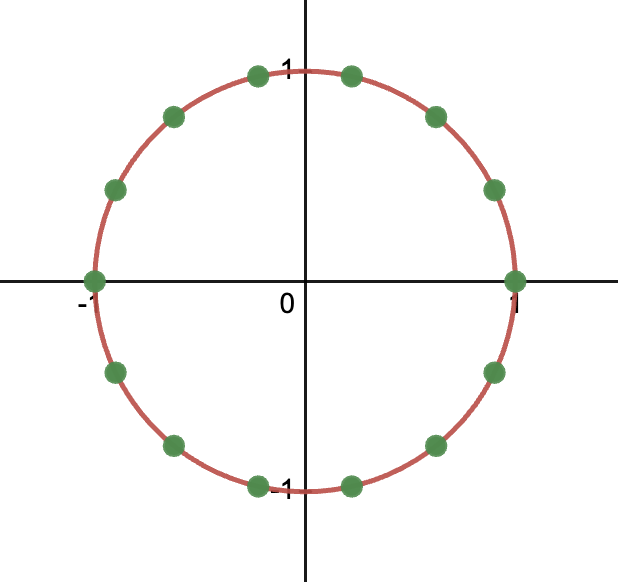
\includegraphics[scale=0.4]{unitcircle.png}
    \caption{The y-values of the above points are $\sin(\frac{k\pi}{m+1})$ for $m=6$, $k=0,1,...,13$. As you can see, there are many duplicates.}
    \label{fig:unit}
\end{figure}

The method used in the implementation is as follows: Suppose we have already calculated $\sin(\frac{k\pi}{m+1})$ for $k=0,1,...,m$, and each value of sine is stored in an array \verb|arr| at the index corresponding to the value of $k$. Note that this array is zero-indexed as opposed to one-indexed, each of these values is positive, meaning it doesn't include every sine value, and that there are many duplicates- for example, $\sin(\frac{(1)\pi}{n+1})=\sin(\frac{((n+1)-1)\pi}{n+1})=\sin(\frac{n\pi}{n+1})$. These were all intentional choices, as they allow us to more easily use modular arithmetic in the following step.

Our goal is to find $s \coloneqq \sin(\frac{ij\pi}{m+1})$ for some $1\leq i,j\leq m$. To find $s$, we take the remainder of $ij$ modulo $2(m+1)$. If the result is less than or equal to $m+1$, then $s$ will be a value on our list- in particular it will be the value at \verb|arr[k]| where $k=(ij)\% (n+1)$. This corresponds to our first identity in $(\dagger)$. If the result is greater than $m+1$, then $s$ will be the negative of a value on our list- in particular the negative of the value at \verb|arr[k]| where again $k=(ij) \% (n+1)$. This corresponds to the second identity in $(\dagger)$.

In the asymmetric case, we then multiply $s$ by $b^{(n-i)/2}c^{(i-1)/2}$, and assign the result to an entry in \verb|eigs| according to \ref{bigboy} and \ref{tritoe}. In the symmetric case, we don't need to bother with multiplying $s$ by a coefficient of $b$ and $c$, since $b=c$ so $b^{(n-i)/2}c^{(i-1)/2}=b^{(n-1)/2}$, which is constant for all $i$. Since every scalar multiple of an eigenvector is also an eigenvector, we can leave out this constant factor and the result will be an eigenvector.

\section{Evaluation Metrics}

Two major methods of evaluation will be used. The first will be the number of floating point operations executed in each run of our implementation, as a function of the size of the matrix. This is a common, if flawed way of measuring algorithmic efficiency. To quote Golub and Van Loan in \textit{Matrix Computations}, ``[f]lop counting is a necessarily crude approach to the measurement of program efficiency since it ignores subscripting, memory traffic, and other overheads associated with program execution. {[...]} Flop counting captures just one dimension of what makes an algorithm efficient in practice."\cite[p.~17]{Golub_Van_Loan_2013} Regardless, it is a common measure of efficiency for the algorithms presented in the book. We will similarly use the number of flops as a rough theoretical estimate of efficiency for the $ATT$ implementations, and compare them against the given flop counts of the ``Practical QR", and ``Symmetric QR" algorithms in Golub/Van Loan.

Also note that to compare the implementations fairly against their theoretical counterparts, we won't be counting flops associated with indexing. Rather we will only count flops that contribute to output values, including those needed to determine the outcome of conditional statements. For example, if the implementation includes a loop \verb|for i in range(n//2)|, we do not count the integer division of $n$ as part of our flop count. We may do this for two reasons: for one, an on-paper description of our algorithm would not mention indices explicitly, and thus would not consider such an operations. Separately, though we are not exactly considering asymptotic runtime complexity, the number of operations done to keep track of indices remains mostly constant as matrix size increases. We will also be making use of certain functions such as \verb|math.sqrt|, \verb|math.pow|, \verb|math.sin|, and \verb|math.cos|. These operations cannot be counted as single floating point operations as there may be more than one flop executed in each call. Even worse, they behave differently depending on the underlying hardware on which they are run. For simplicity, we will count the first two of these as \textit{power operations} and the second two as \textit{trig operations} and keep track of them in separate categories. Again, Golub/Van Loan sets the precedent for this, as the authors often track the number of necessary square roots separately from the number of flops. \cite{Golub_Van_Loan_2013}

To get a better and more practical measurement of the algorithm's efficiency, we will also run empirical tests. We begin by randomly generating a set of ATT test matrices of sizes 3 through 102, with real entries between $-100$ and 100. In the asymmetric case, I decided to keep the entries $b$ and $c$ nonnegative, so that the eigenvalues would be real- I mostly did this as my implementation relies on the \verb|math.pow| function in Python, which cannot handle complex numbers. We generate 1000 matrices of each size: 500 symmetric, and 500 asymmetric. We pass each asymmetric matrix to \verb|PentaEigvals| and \verb|PentaEigvecs|, and each symmetric matrix to \verb|SymmPentaEigvals| and \verb|SymmPentaEigvecs|, and for each execution, record the time it takes for the function to return a value. We also pass each matrix to the functions in \verb|numpy.linalg| which perform analogous operations, and similarly record the time it takes for each to return a value. For each function and each size of matrix, we average all 500 recorded times and record that as our evaluation of the function's performance for that size of matrix.

Numpy provides the best option for a standard test because it are the most commonly used linear algebra library in Python. The framework provided by Numpy is very accessible and allows me to more easily implement my algorithm and give more attention to detail where possible. Moreover it is well-optimized and provide a way for me to test my algorithm against a commonplace standard.

The analogous functions in \verb|numpy.linalg| are as follows: \verb|np.linalg.eigvals| finds the eigenvalues of a general matrix, \verb|np.linalg.eigvalsh| finds the eigenvalues of a symmetric matrix, \verb|np.linalg.eig| finds the eigenvectors of a general matrix, and \verb|np.linalg.eigh| finds the eigenvectors of a symmetric matrix. To actually perform these computations, \verb|numpy| implements a wrapper for the \textit{LAPACK} library of subroutines, which is written in Fortran 90. \cite{np.LA} In other words, all of the actual computation executed by these four functions is done in Fortran, whereas my implementation does all of its computation natively in Python As such, this is not an ideal comparison- however due to my inexperience with Fortran, I believe this is my best option. As Python is an interpreted language whereas Fortran is compiled, we make the assumption that any computation executed in Python is slower than an analogous computation in Fortran. As a result, if the tests of one of my functions run \textit{as fast as or faster than} the test of the analogous function in \verb|numpy.linalg|, we will conclude that the function would run faster in Fortran as well, and we will consider this a success. If the test of any of my functions runs slower than the test of the analogous method in \verb|numpy.linalg|, we will say that the test is inconclusive.

\section{Evaluation Results and Discussion}

\subsection{Floating-Point Operations}

\subsubsection{Eigenvalues}

Recall that the only major difference between eigenvalue algorithms is a change in the way a certain constant is calculated. In the asymmetric case, this is calculated as \verb|2*math.sqrt(b*c)|, which we are counting as two flops and one power operation. In the symmetric case, this is calculated as \verb|abs(b+b)|, for only one flop. We do not count the execution of \verb|abs()| as a flop, as it is essentially a comparison operation. \cite{Gray_2017}

Other than that, the symmetric and asymmetric cases are the same, but the runtimes are different depending on whether the size of the matrix $n$ is odd or even. If $n$ is even, we run the following snippet $\frac{n}{2}$ times: \verb|a+const*math.cos((i+1)*math.pi/((n//2)+1))|. This contains 7 flops and one trig function.

If $n$ is odd, we run the same snippet $\lfloor\frac{n}{2}\rfloor$ times, as well as the following snippet a total of $\lceil\frac{n/2}\rceil$ times: \verb|a+const*math.cos((j+1)*math.pi/((n//2)+2))|. Through similar analysis, this snippet contains 7 flops and one trig function.

Thus, \verb|PentaEigvals()| runs in $\frac{7}{2}n+2$ flops, one power operation, and $\frac{n}{2}$ trig operations if $n$ is even, and $7n+2$ flops, one power operation, and $n$ trig operations if $n$ is odd. Furthermore, \verb|SymmPentaEigvals()| runs in $\frac{7}{2}n+1$ and $\frac{n}{2}$ trig operations if $n$ is even, and $7n+1$ flops and $n$ trig operations if $n$ is odd.

By comparison, the Practical QR eigenvalue algorithm in Golub/Van Loan requires about $10n^3$ flops, and the Symmetric QR eigenvalue algorithm takes about $\frac{4}{3}n^3$ flops, though the divide-and-conquer algorithm is not the one outlined in the description of the algorithm. A different source\cite{Arbenz_2018} explicitly calculates the runtime of Cuppen's divide-and-conquer method, and also gets $\frac{4}{3}n^3$ flops.

\subsubsection{Eigenvectors}

We begin with \verb|PentaEigvecs()|, and again we will have different runtimes based on the parity of $n$. 

If $n$ is even, we generate sine values by running the following snippet $\frac{n}{2}$ times:
\verb|math.sin(i*math.pi/((n//2)+1))|. This is 4 flops and one trig operation per execution. We then generate our coefficients by running the following snippet $\frac{n}{2}$ times: \verb|coeff=math.pow(b,((n//2)-((i//2)+1))/2)| \verb|*math.pow(c,(i//2)/2)|. This amounts to 7 flops and two power operations. Finally, we assign the sine values to our matrix. We do this by running a loop that executes $\frac{n}{2}\frac{n}{2}=\frac{n^2}{4}$ times, and contained in the loop is an \verb|if| statement with condition \verb|(((i//2)+1)*(j+1)) % (n+2) > (n//2)+1|. To compute the result of the condition each time requires 8 flops - the modulus operator is counted as a flop, and the comparison operator is disregarded. Regardless of the outcome of the comparison, we will always execute the snippet \verb|(((i//2)+1)*(j+1)) % ((n//2)+1)| for 7 flops- this specifies which value of sine we want to use. We then multiply the result by \verb|coeff| for a total of 8 flops. Depending on the outcome of the comparison, we may also multiply by $-1$ for a total of 9 flops. It's not entirely clear how often multiplication by $-1$ happens or if this frequency is easy to find, so for simplicity we will assume that 9 flops are performed for every iteration of the if statement. All told, if $n$ is even then \verb|PentaEigvecs()| performs approximately $\frac{9}{4}n^2+\frac{11}{2}n$ flops, $n$ power operations, and $\frac{n}{2}$ trig operations.

If $n$ is odd, then similarly to the eigenvalue methods, we run all the same code as above, but replace each $\frac{n}{2}$ with an $n$. This gives a total of $9n^2+11n$ flops, $2n$ power operations, and $n$ trig operations.

In the symmetric case, everything behaves identically, except that we don't calculate \verb|coeff|. This removes all the power operations involved, removes all 7 flops associated with each computation of \verb|coeff|, and removes one flop for each execution of the \verb|if| statement. So \verb|SymmPentaEigvecs()| performs $2n^2+2n$ flops and $\frac{n}{2}$ trig operations if $n$ is even, and $8n^2+4n$ flops and $n$ trig operations if $n$ is odd.

By comparison, the Practical QR eigenvector algorithm in Golub/Van Loan requires about $25n^3$ flops, and the Symmetric QR eigenvector algorithm takes about $9n^3$ flops.

\subsection{Empirical Tests}

In this section, we detail the results of the tests conducted as outlined in the previous section. The graphs of our results are given in Figures \ref{aval}, \ref{sval}, \ref{avec}, and \ref{svec}.

    \begin{figure}[h!]
    \centering
    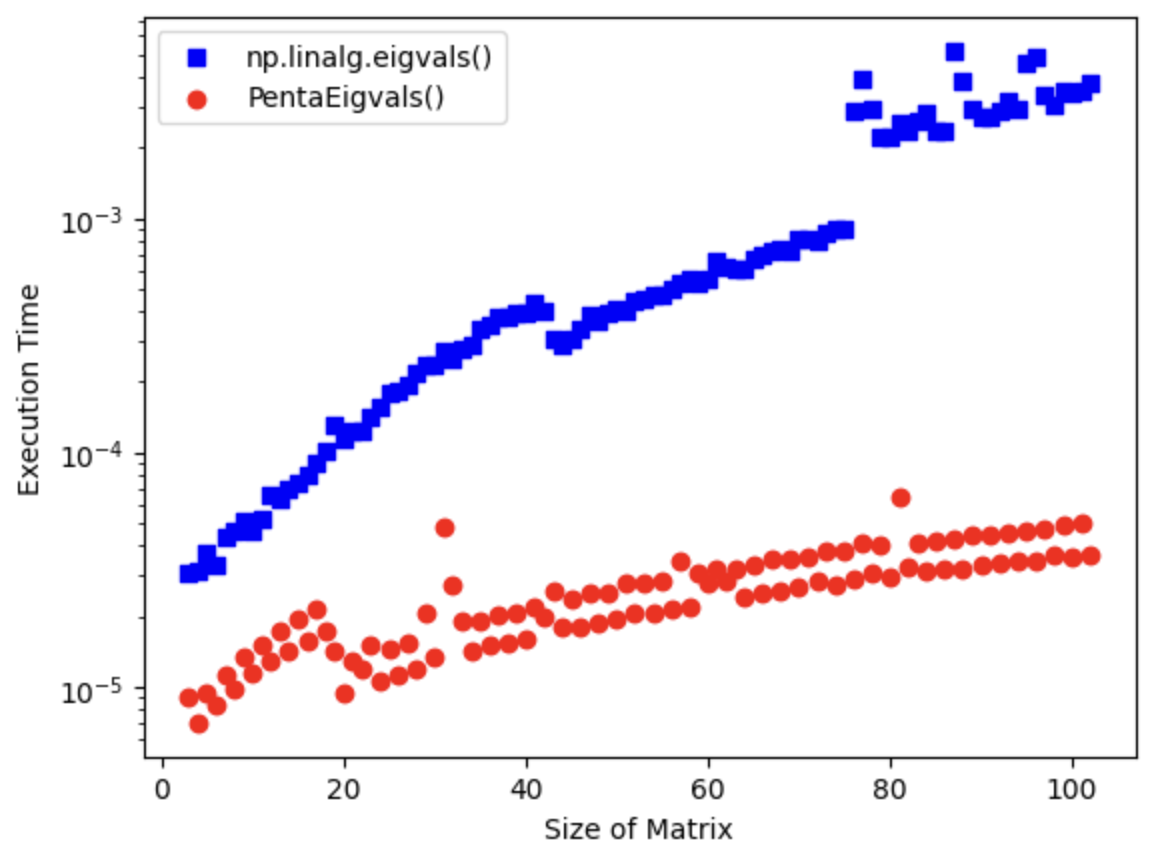
\includegraphics[scale=0.35]{aval.png}
    \caption{Comparing functions for asymmetric eigenvalues (note the log scale on the vertical axis)}
    \label{aval}
\end{figure}
\begin{figure}[h!]
    \centering
    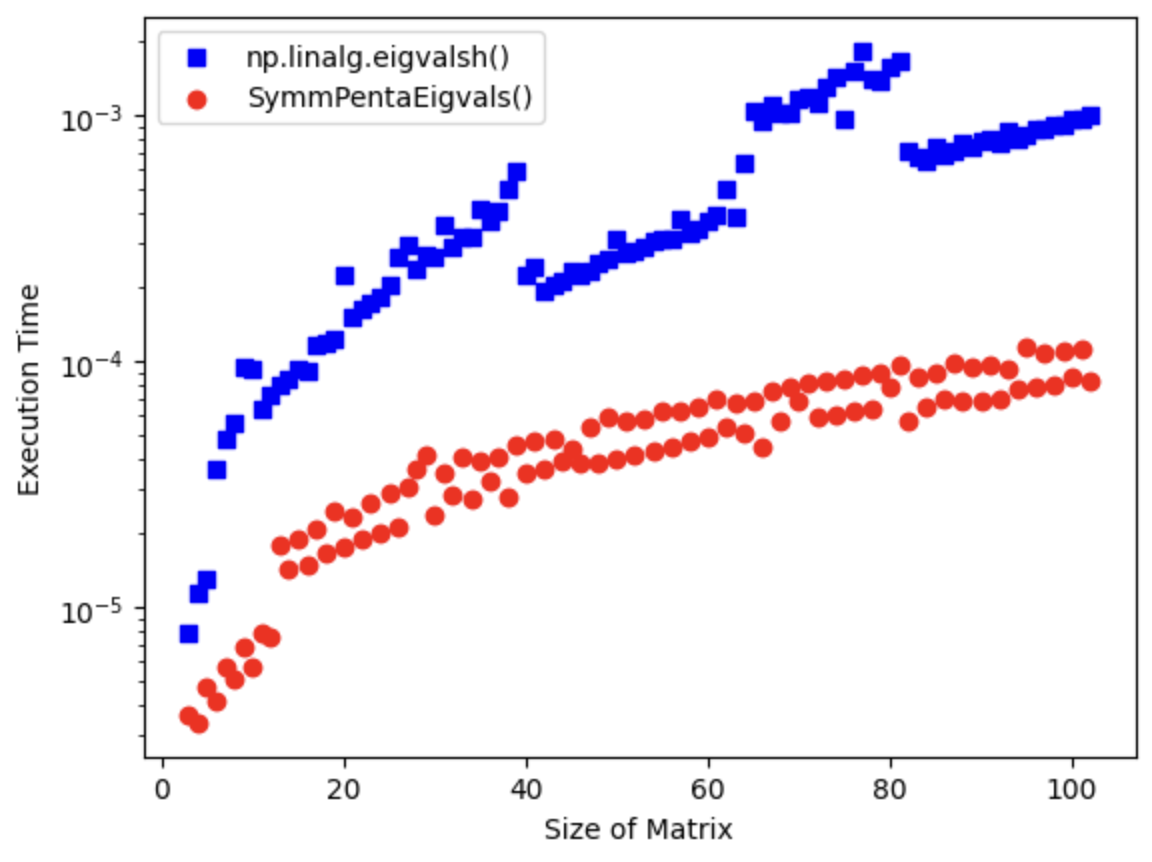
\includegraphics[scale=0.35]{sval.png}
    \caption{Comparing functions for symmetric eigenvalues (note the log scale on the vertical axis)}
    \label{sval}
\end{figure}
\begin{figure}[h!]
    \centering
    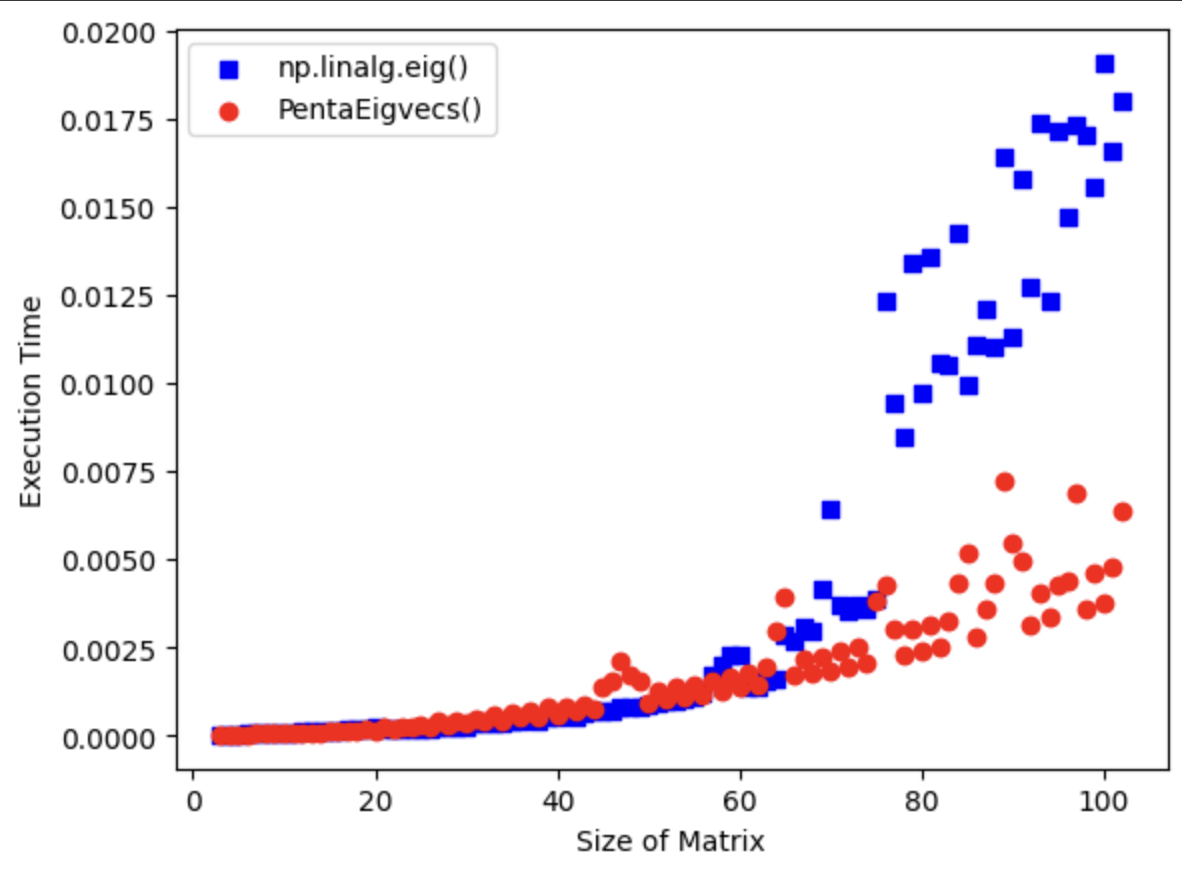
\includegraphics[scale=0.35]{avec.png}
    \caption{Comparing functions for asymmetric eigenvectors}
    \label{avec}
\end{figure}
\begin{figure}[h!]
    \centering
    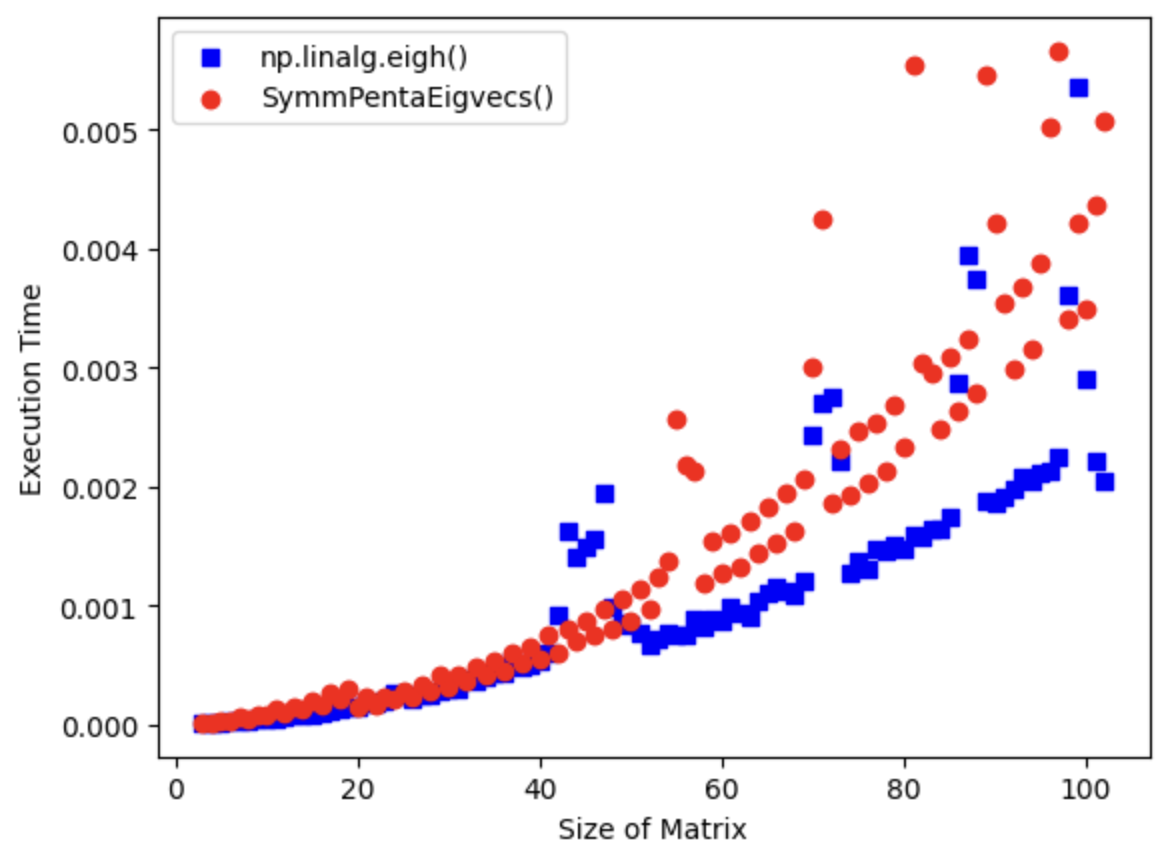
\includegraphics[scale=0.35]{svec.png}
    \caption{Comparing functions for symmetric eigenvectors}
    \label{svec}
\end{figure}

\subsection{Discussion}

We begin with flop comparisons. The number of flops explicitly counted in each of our four implementations is far lower than the given flop counts for the QR algorithms, especially asymptotically. However whether the total number of flops is lower depends on the assumptions made about the number of flops performed during power and trig operations. If we make the assumption that the number of flops is constant, we have that our $ATT$ implementations take asymptotically far fewer flops than their QR counterparts. 

The runtime graphs for the eigenvalue algorithms seem to support this, with \verb|PentaEigvals()| performing orders of magnitude better than its QR counterpart and \verb|SymmPentaEigvals()| always staying below the Symmetric QR as well. In all the graphs there are two distinct lines- one corresponding to each parity of matrix size. In both eigenvalue algorithms, both lines stay well ahead of the competition, and these algorithms are unequivocally successful.

However, the eigenvector graphs tell a different story. \verb|PentaEigvecs()| performs on par with the general QR eigenvector algorithm for most of the sampled matrix sizes- that is, until around $n=64$, at which point it begins to do much better. My suspicion for \verb|eig()|'s sudden blowup in time is that matrices have to be stored differently in memory- its likely that the instance of Colab in which these tests were executed had 64-bit registers and the transfer of memory for the purpose of the QR algorithm became more complicated and less predictable with larger matrix sizes. \verb|PentaEigvecs()| did not have a similar blowup in memory- I'm not sure why, but its definitely true that less matrix processing and editing was required- we only create and output a single $n\times n$ matrix.

\verb|SymmPentaEigvecs()| similarly performs on par with \verb|eigh()| for small matrix sizes, but begins to lag behind for larger ones. Unlike \verb|eig()|, \verb|eigh()| has no sudden blowup in time at $n=64$. My best guess for why it remains consistent is that tridiagonal matrices are stored differently than other matrices in LAPACK, being represented as a trio of $n$-long vectors instead of a full matrix. Other than that, the lower constant factor seems to have given it the edge over \verb|SymmPentaEigvecs()|. 

This also calls into question the apparent success of \verb|PentaEigvecs|, as it's not clear whether or not it would have beaten \verb|eig()| for larger matrix sizes if the suspected storage issues had not been present. Our flop count suggests that both \verb|PentaEigvecs| and \verb|SymmPentaEigvecs| should be asymptotically faster than their counterparts, but it's possible that for that to happen for \verb|SymmPentaEigvecs()| with our testing setup, we would need to test the algorithm for larger matrix sizes than we are able to deal with. For these reasons, we conclude that our tests for \verb|PentaEigvecs()| and \verb|SymmPentaEigvecs()| are both inconclusive.

\section{Ethical Considerations}

The ethics of any project are obviously important to consider. When developing a tool, it's important to think about how others will use the tool, whether or not they can use it to bring about harm, and especially whether the design of the tool enables them to do so or may unintentionally cause harm during regular use. 

The tool that I am developing is unfortunately so abstract that it is difficult if not impossible for me to effectively gauge how it could bring about harm. It is so specific and low-level in its application that I have no control over how someone else might use this algorithm to cause harm or perpetuate inequity. I am not drawing upon data sets that may skew results, and I am not including features which fit in a larger societal context. My tool is not even designed to be used by a general audience, but by those interested in optimizing linear algebraic computations. As such I see no way in which I could realistically mitigate societal inequity in my algorithm- that will be the responsibility of those who want to use it for another purpose.

\section{Future Work, and Conclusion}

The presented method of computing the eigenvalues of $ATT$ matrices was shown to be much faster than other commonly-used eigenvalue methods. Our presented methods for computing the eigenvectors of $ATT$ matrices were shown to be faster on paper- however in practice, it was unclear whether or not our method outperformed its counterparts. 

Research in this area could continue in many directions. A first and obvious step is implementing these methods in an environment where they can be directly compared to modern eigensystem methods, i.e. in Fortran 90 for comparison directly against LAPACK. Furthermore, the implementation could include support for complex eigenvalues and matrices with complex entries to achieve a more general analysis.

Another direction is to integrate the divide-and-conquer method into the symmetric version of our method. When we find the eigenvalues of an ATT matrix, we implicitly examine a tridiagonal Toeplitz matrix- if that matrix is symmetric we could incorporate the principles of Cuppen's divide-and-conquer algorithm to derive a new method. It's not out of the question that the principles of divide-and-conquer could be applied to general pentadiagonal Toeplitz matrices to develop a new algorithm or formula for its eigenvalues.

\appendix
\section{Replication Instructions and Code Architecture}

The code for this project is accessible at \url{https://github.com/hall-nate/NJHSeniorComps}. The code itself is stored as a Google Colab notebook, and can be opened easily in Colab directly from Github. 

Dependencies for this project are the Numpy and Matplotlib libbraries.

There are two code blocks: the first has the definitions for all four functions mentioned in this paper: \verb|PentaEigvals|, \verb|SymmPentaEigvals|, \verb|PentaEigvecs|, and \verb|SymmPentaEigvecs|. It also has two functions which generate pseudo-random ATT matrices- these are \verb|RandPentaMtx| and \verb|RandSymmPentaMtx|. 

If working in Colab, simply run each block. Working in Colab is especially recommended as it has all dependencies preinstalled. If you would prefer to run the project on your home environment, the results of the tests may also very depending on whether you have a Fortran compiler or any specialized matrix libraries, such as OpenBLAS or ATLAS, installed. You can run all tests as one Python script, or create separate files for the function definitions and tests.
 
\printbibliography


\end{document}
